\documentclass[12pt,a4paper]{report}

\usepackage[a4paper,margin=1in]{geometry}
\usepackage[T1]{fontenc}
\usepackage[utf8]{inputenc}
\usepackage{mathptmx}
\usepackage{setspace}
\usepackage{graphicx}
\usepackage{float}
\usepackage{booktabs}
\usepackage{array}
\usepackage{tabularx}
\usepackage{longtable}
\usepackage{pdflscape}
\usepackage{caption}
\usepackage{csquotes}
\usepackage{xcolor}
\usepackage{listings}
\usepackage[hidelinks]{hyperref}

\usepackage[
  backend=biber,
  style=apa,
  sorting=nyt
]{biblatex}

\addbibresource{references.bib}

\graphicspath{{../elements/}{figures/}{diagrams/img/}}

\setlength{\parindent}{0pt}
\setlength{\parskip}{0.75em}
\setlength{\emergencystretch}{2em}
\onehalfspacing

\makeatletter
\renewcommand{\@makechapterhead}[1]{%
  \vspace*{1.5em}%
  {\parindent \z@ \raggedright \normalfont
    \Huge\bfseries #1\par\nobreak
    \vskip 1.8em}}
\renewcommand{\@makeschapterhead}[1]{%
  \vspace*{1.5em}%
  {\parindent \z@ \raggedright \normalfont
    \Huge\bfseries #1\par\nobreak
    \vskip 1.8em}}
\makeatother

\newcommand{\projecttitle}{Development of a Machine Learning-Based System for Cardiopulmonary Sound Separation}
\newcommand{\shorttitle}{HealthTech}
\newcommand{\coursename}{CSE6234 Software Design}
\newcommand{\groupname}{Group 1}
\newcommand{\tutorialsection}{TT5L}
\newcolumntype{Y}{>{\raggedright\arraybackslash}X}
\definecolor{codegreen}{RGB}{120,220,160}
\definecolor{codecyan}{RGB}{110,210,255}
\definecolor{codeorange}{RGB}{255,190,120}
\definecolor{codegray}{RGB}{210,210,210}
\definecolor{codeblack}{RGB}{20,20,20}

\lstdefinestyle{reportPython}{
  language=Python,
  backgroundcolor=\color{codeblack},
  basicstyle=\ttfamily\small\color{white},
  keywordstyle=\color{codecyan}\bfseries,
  commentstyle=\color{codegreen},
  stringstyle=\color{codeorange},
  numberstyle=\tiny\color{codegray},
  breaklines=true,
  breakatwhitespace=false,
  columns=fullflexible,
  keepspaces=true,
  showstringspaces=false,
  frame=single,
  framerule=0pt,
  rulecolor=\color{codeblack},
  xleftmargin=0.5em,
  xrightmargin=0.5em,
  aboveskip=1em,
  belowskip=1em
}
\lstset{style=reportPython}

\begin{document}
\hypersetup{pageanchor=false}

\begin{titlepage}
  \centering

  \begin{minipage}{0.65\textwidth}
    \centering
    \IfFileExists{../elements/FCI__MMU_LOGO.png}{%
      
\includegraphics[width=\linewidth,height=2.4cm,keepaspectratio]{../elements/FCI__MMU_LOGO.png}%
    }{%
      \fbox{FCI logo placeholder}%
    }
  \end{minipage}

  \vspace{2.5cm}

  {\Large \coursename\par}
  \vspace{0.8cm}
  {\Large Software Design Proposal and Software Design Pattern Document\par}
  \vspace{1.2cm}
  {\huge\bfseries \shorttitle\par}
  \vspace{0.8cm}
  {\Large\bfseries \projecttitle\par}

  \vfill

  {\large \groupname\par}
  {\large Tutorial Section: \tutorialsection\par}

  \vspace{0.8cm}

  \begin{tabular}{ll}
    \toprule
    \textbf{Name} & \textbf{Student ID} \\
    \midrule
    AL-SALOUL, ASHRAF ALI HUSSEIN & 1221303805 \\
    AHMAD AKMAL ASYRAAF BIN SHAMS & 242UC244CJ \\
    RESHMA A/P KRISHNAMURTHY & 243UC247KW \\
    SHARWIN A/L R SIVALINGAM & 241UC241C1 \\
    \bottomrule
  \end{tabular}

  \vfill

  {\large \today\par}
\end{titlepage}

\clearpage
\hypersetup{pageanchor=true}
\pagenumbering{roman}
\tableofcontents
\clearpage

\chapter*{Abstract / Executive Summary}
\addcontentsline{toc}{chapter}{Abstract / Executive Summary}
This report presents a software design proposal and design pattern document for a HealthTech cardiopulmonary sound separation prototype. The proposed system accepts mixed WAV audio, uses NeoSSNet to separate the recording into heart sound and lung sound outputs, stores structured metadata and processing records in SQLite, and keeps uploaded and generated audio files in local storage.

The report focuses on software design rather than clinical validation. It documents the problem statement, objectives, system scope, UML models, requirements, design principles, and selected design patterns. FastAPI is used as the backend API layer, SQLite supports jobs, results, logs, and metadata, and the local filesystem stores audio artifacts and model files. The Facade, Strategy, and Factory Method patterns are proposed to simplify the separation workflow, isolate algorithm execution behind a strategy context, and create upload audio validators through a Creator and ConcreteCreator structure.

\clearpage
\pagenumbering{arabic}

\chapter{Introduction}

\section{Executive Summary / Abstract}

This report presents a software design proposal and design pattern document for a cardiopulmonary sound separation system. The proposed system is a HealthTech prototype that accepts mixed WAV audio and separates it into heart sound and lung sound outputs using NeoSSNet. The project is designed as a local web-based application with a FastAPI backend, a simple HTML/CSS/JavaScript interface, SQLite database storage for metadata and processing records, and local filesystem storage for uploaded and generated audio files.

The purpose of the system is to demonstrate how machine learning inference can be integrated into a reusable software system rather than being kept only as an isolated model script. The application supports upload, validation, real separation, output preview, download, and processing history. This document focuses on software design quality, including requirements, UML modelling, database structure, layered architecture, and design patterns. The prototype is not a clinical diagnosis system and does not claim clinical validation. Instead, it is intended to show a practical and explainable software design for cardiopulmonary sound separation.

\section{Background / Introduction}

Cardiopulmonary sound recordings often contain both heart and lung components because the two sound sources are captured from nearby areas of the chest. In a mixed recording, the sound of one organ can interfere with analysis of the other. This creates a useful software engineering problem: the system must accept an input audio file, apply a sound separation model, produce separate heart and lung audio outputs, and keep the processing records traceable for review.

Recent research has shown that computational methods can support heart and lung sound processing, including source separation and deep learning-based heart sound analysis. However, a model alone is not enough for a usable application. A student, lecturer, researcher, or demonstration user needs a complete workflow that includes file upload, validation, inference, storage, result preview, download, error handling, and history. For this reason, the project is framed as a software design assignment that connects machine learning with maintainable backend and frontend architecture.

The proposed system uses NeoSSNet as the core separation model and stores model-related files in local storage. SQLite is used to store structured data such as uploaded audio metadata, model records, separation jobs, result paths, metrics, and logs. The actual WAV audio files are stored on the filesystem so that the database remains lightweight and easy to inspect. This separation between database records and audio artifacts supports a practical local deployment suitable for a Final Year Project prototype.

\section{Problem Statement}

Mixed cardiopulmonary audio is difficult to use directly when the target task requires separate heart and lung sound outputs. If a system only stores uploaded mixed audio, users cannot easily preview the isolated components or use them for later analysis and demonstration. At the same time, if separation is implemented only as a standalone script, the workflow may lack upload handling, database tracking, result retrieval, logging, and a clear user interface.

The project therefore needs a reusable software system that can connect audio upload, NeoSSNet inference, file storage, SQLite metadata, and browser-based result viewing. The design must remain simple enough for a student project, but structured enough to explain through software design concepts, UML diagrams, and design patterns. The system must not present separated audio as clinical diagnosis; it should be described as a prototype that demonstrates automated cardiopulmonary sound separation and supporting software architecture.

\section{Project Objectives}

The objectives of this project are:

\begin{enumerate}
  \item To design a local web-based system that accepts mixed cardiopulmonary WAV audio through a browser interface.
  \item To validate uploaded audio files before they are stored or processed by the backend.
  \item To integrate NeoSSNet as the real cardiopulmonary sound separation model for generating heart and lung output audio.
  \item To save separated heart and lung WAV files in local output folders for preview and download.
  \item To store structured metadata, job records, result paths, logs, and optional evaluation metrics in SQLite.
  \item To provide result viewing, audio preview, download support, and processing history through the web interface.
  \item To document a maintainable software design using UML diagrams, requirements, design principles, and selected design patterns.
\end{enumerate}

\subsection{Literature Review}

Cardiopulmonary sound analysis studies information contained in heart and lung recordings, where useful physiological sounds may overlap because both sources are captured from the chest area. In practical recordings, the heart component can interfere with lung sound analysis, while lung sounds and breathing noise can also obscure heart sound patterns. Sound separation is therefore an important preprocessing and application problem because it attempts to recover clearer heart and lung signals from a mixed recording. For the proposed HealthTech prototype, the literature is relevant not only because it motivates machine learning-based separation, but also because it shows the need for a usable software system around the algorithm. A practical system must support upload, validation, inference, storage, preview, download, and processing history rather than treating separation as an isolated research script.

Recent studies show two complementary technical directions. The first is deep learning-based source separation. NeoSSNet has been proposed for real-time neonatal chest sound separation, with the aim of separating mixed chest sound recordings into heart and lung components \parencite{poh2024neossnet}. Its audio source separation approach is directly aligned with this project because the application must generate two usable WAV outputs: one heart sound file and one lung sound file. NeoSSNet also motivates the software architecture because its inference process can be placed behind a dedicated machine learning boundary and called from the backend service layer. However, the research contribution mainly concerns the model and separation performance. It does not by itself provide a complete application workflow for user upload, database-backed job tracking, browser preview, or maintainable backend organization.

The second direction is hybrid separation using signal processing and decomposition methods. A DAE--NMF--VMD method has been studied for separating heart and lung sounds by combining deep autoencoder-based representation learning, nonnegative matrix factorization, and variational mode decomposition \parencite{sun2024daenmfvmd}. Compared with a neural separation model such as NeoSSNet, this approach shows that cardiopulmonary sound separation can also be designed as a multi-stage processing pipeline. This comparison is useful for the proposed system because future versions may need to compare algorithms with different preprocessing steps, configuration parameters, model files, and output handling. Therefore, the software should avoid embedding one algorithm too deeply into route logic. A modular design with an interchangeable algorithm interface is better suited for future experimentation while keeping the current prototype focused on NeoSSNet.

Broader deep learning work in heart sound analysis further supports the need for careful system design. Deep learning techniques, datasets, and applications for heart sound analysis have been reviewed across preprocessing, feature extraction, model development, and potential clinical application areas \parencite{zhao2024heartanalysis}. This wider literature shows the growing importance of intelligent biomedical sound processing, but it also highlights concerns such as dataset limitations, generalisation, and the need for further refinement before broad clinical use. These points are important for this report because the proposed system should not be presented as a clinically validated diagnostic tool. It is more accurately described as a proof-of-concept HealthTech software prototype that demonstrates cardiopulmonary sound separation and the supporting software architecture needed to make the workflow usable and traceable.

Taken together, the studies show that cardiopulmonary sound separation and heart sound analysis have promising algorithmic foundations, but they also reveal a software design gap. Existing work focuses strongly on algorithms, while less attention is given to reusable application architecture for a local prototype. In particular, the literature does not fully address database-backed processing history, structured metadata, user upload workflow, separated audio preview and download, local file storage, logging, and maintainability through design patterns. The proposed system responds to this gap by combining FastAPI for the backend API, SQLite for metadata and job records, local filesystem storage for uploaded and separated WAV files, and NeoSSNet for real separation. This design connects research-level separation models with a practical software workflow that can be demonstrated, inspected, and extended in a student software design assignment.

\section{Project and System Scope}

\subsection{In Scope}

The project scope covers a local prototype that accepts mixed WAV audio, validates the file, stores the uploaded audio in a local folder, runs NeoSSNet-based separation, generates separated heart and lung WAV outputs, stores output files locally, records metadata and job status in SQLite, and provides browser-based preview, download, and processing history. The report also covers software design artefacts such as use case modelling, class modelling, database modelling, requirements, design principles, and design patterns.

The dataset and runtime storage are treated as separate concerns. Dataset files such as HLS-CMDS data are used for development or evaluation purposes, while runtime uploads and generated outputs are stored under the application storage folders. This separation avoids mixing training or testing data with user-uploaded demo files.

\subsection{Out of Scope}

The project does not aim to provide medical diagnosis, clinical decision support, hospital deployment, or validated clinical accuracy. It does not claim that separated audio is suitable for real clinical use without further testing and approval. Authentication, cloud deployment, multi-user role management, and production-scale monitoring are also outside the current scope unless they are added in a later phase.

Training a new model from runtime uploads is also outside the current system scope. Runtime uploads are used for inference and demonstration only. The current design focuses on integrating real NeoSSNet inference into a clean software system that is practical for local execution and clear enough to defend in a software design presentation.

\chapter{System Overview}

The proposed system is a local web-based prototype for cardiopulmonary sound separation. A user uploads a mixed WAV audio file through the browser interface, and the FastAPI backend validates the upload, stores the original file, creates database records, runs NeoSSNet separation, saves the separated heart and lung audio files, and returns results for preview and download. SQLite is used for structured records such as uploaded audio metadata, model information, separation jobs, result paths, metrics, and logs, while local folders are used for the actual audio files and model checkpoints.

The following diagrams describe the system from different software design viewpoints. The use case diagram presents the system functions from the user's perspective, the class diagram shows the planned software components, the entity relationship diagram shows the database structure, and the object diagram gives an example of one completed separation job.

\section{Generic Use Case}

\begin{figure}[H]
  \centering
  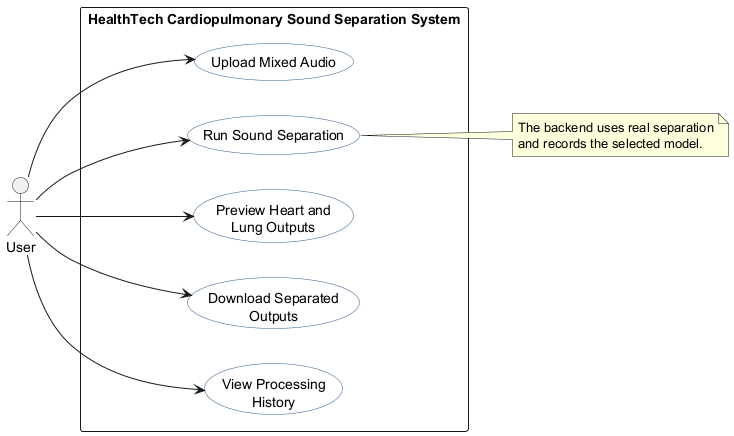
\includegraphics[width=0.95\textwidth]{use_case_diagram.png}
  \caption{Generic Use Case Diagram}
  \label{fig:generic-use-case}
\end{figure}

Figure~\ref{fig:generic-use-case} shows the main actions available to a single generic actor, the User. The diagram is intentionally simple because the same user-facing workflow can be demonstrated by a student, lecturer, examiner, or researcher without changing the system boundary. The central use cases are uploading mixed audio, running cardiopulmonary sound separation, previewing separated heart and lung outputs, downloading separated outputs, and viewing processing history.

The simplified diagram keeps internal responsibilities such as validation, model selection, metadata storage, and logging out of the actor view. Those responsibilities are still required by the backend, but they support the visible workflow rather than appearing as separate user goals. This makes the use case model easier to read while still showing how upload, separation, preview, download, and history are connected.

\begin{landscape}
\begin{table}[H]
  \centering
  \scriptsize
  \setlength{\tabcolsep}{2pt}
  \caption{Use Case Descriptions}
  \label{tab:use-case-descriptions}
  \begin{tabular}{@{}p{0.11\linewidth} p{0.06\linewidth} p{0.15\linewidth} p{0.12\linewidth} p{0.15\linewidth} p{0.13\linewidth} p{0.13\linewidth}@{}}
    \toprule
    \textbf{Use Case Name} & \textbf{Actor} & \textbf{Description} & \textbf{Precondition} & \textbf{Main Flow} & \textbf{Alternative Flow} & \textbf{Postcondition} \\
    \midrule
    Upload Mixed Audio & User & Uploads a mixed cardiopulmonary WAV file through the browser interface. & The user has a supported WAV file. & The user selects a file and submits it; the backend validates and stores the upload. & If the file is invalid, the system rejects it and shows an error message. & Uploaded audio metadata and file path are stored. \\
    Run Sound Separation & User & Starts separation for an uploaded audio file using the selected or active model. & A valid uploaded audio record exists. & The user starts separation; the backend creates a job, runs the model, and stores output metadata. & If processing fails, the job is marked failed and the error is logged. & Heart and lung output files are generated for a successful job. \\
    Preview Separated Audio & User & Plays the separated heart and lung outputs in the browser. & A separation job has completed successfully. & The user opens the result view and plays the available audio controls. & If a file is missing or unsupported by the browser, the system keeps the download option available. & The user can inspect the separated outputs without leaving the interface. \\
    Download Separated Audio & User & Downloads the generated heart and lung WAV files. & A completed result contains valid output paths. & The user selects the heart or lung download link. & If the requested file is unavailable, the system returns a clear error response. & The selected separated audio file is saved by the user's browser. \\
    View Processing History & User & Reviews previous uploads, jobs, statuses, models, and result links. & At least one upload or job record exists, or the history list may be empty. & The user opens the history section and the system loads stored records from SQLite. & If no records exist, the system displays an empty history state. & The user can trace previous processing activity and reopen results. \\
    \bottomrule
  \end{tabular}
\end{table}
\end{landscape}

\section{Class Diagram}

\begin{landscape}
\begin{figure}[H]
  \centering
  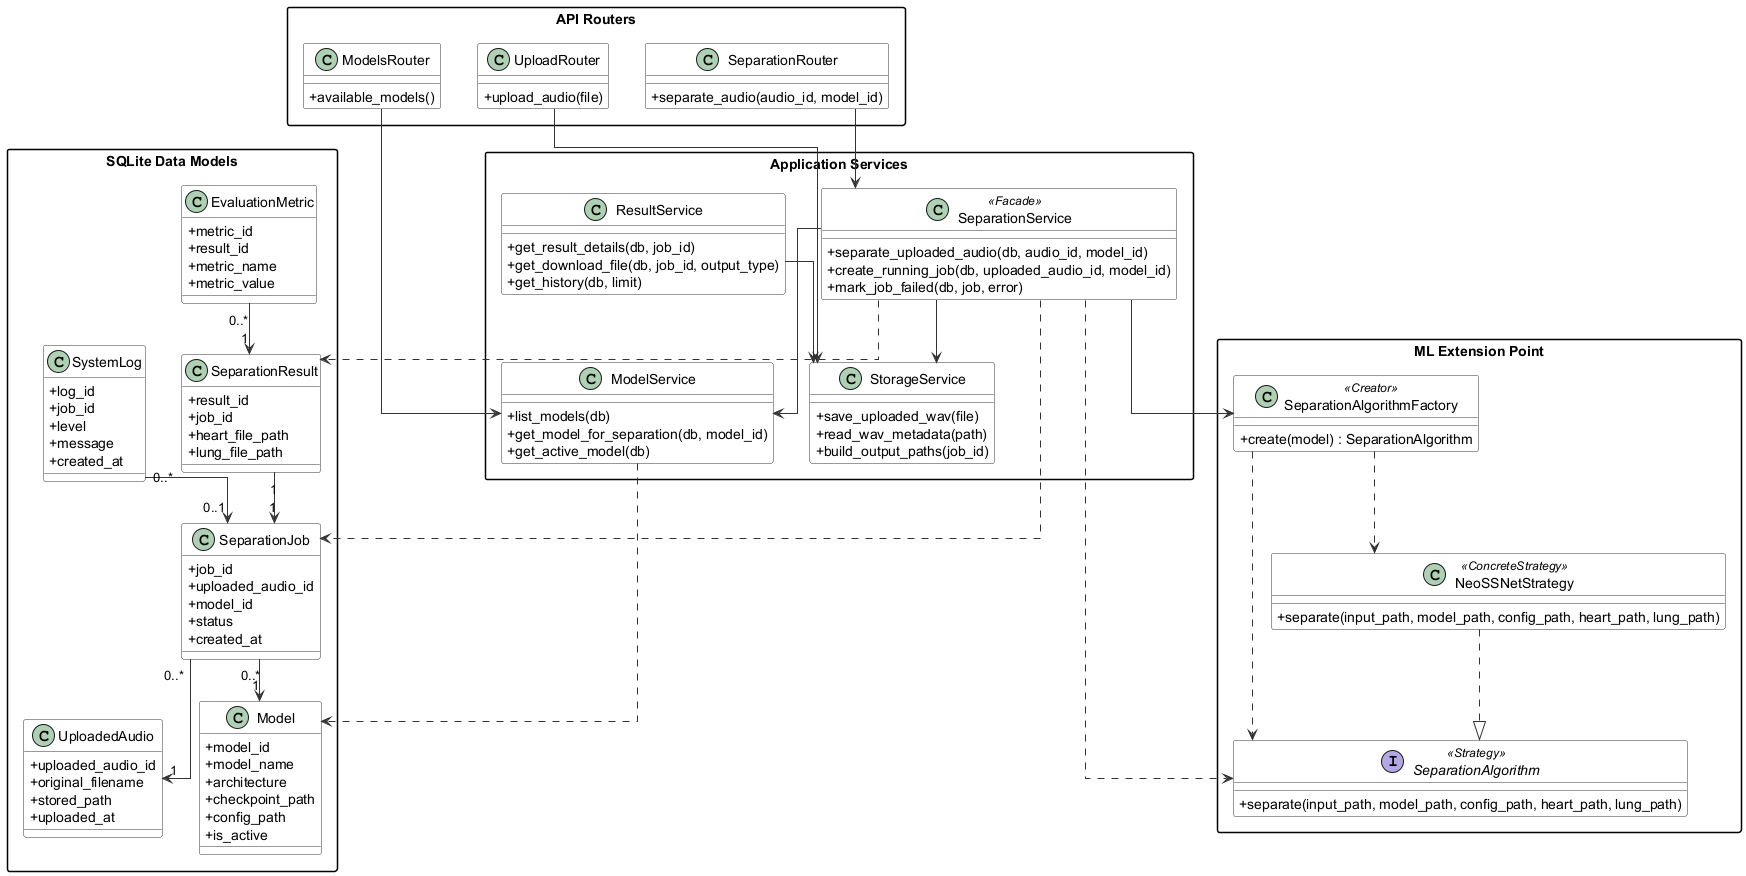
\includegraphics[width=1.25\textwidth]{overall_class_diagram.png}
  \caption{Overall System Class Diagram}
  \label{fig:overall-class-diagram}
\end{figure}
\end{landscape}

Figure~\ref{fig:overall-class-diagram} presents the planned software classes grouped into frontend, router, service, machine learning, and persistence responsibilities. The browser interface calls FastAPI routers, the routers delegate work to service classes, and the service layer coordinates storage, model selection, algorithm creation, machine learning inference, and SQLite result records.

The class diagram also identifies where the selected design patterns are located:
\begin{itemize}
  \item \texttt{SeparationService} is the Facade because it presents one separation workflow to the router.
  \item \texttt{SeparationAlgorithm} and \texttt{NeoSSNetStrategy} form the Strategy structure because the service calls the algorithm through an abstraction.
  \item \texttt{SeparationAlgorithmFactory} is the Factory Method component because it creates the correct algorithm object from the selected model record.
\end{itemize}
This design keeps upload, separation, storage, result viewing, and history modular while avoiding hardcoded NeoSSNet logic in the router.

\section{Entity Relationship Diagram (ERD)}

\begin{figure}[H]
  \centering
  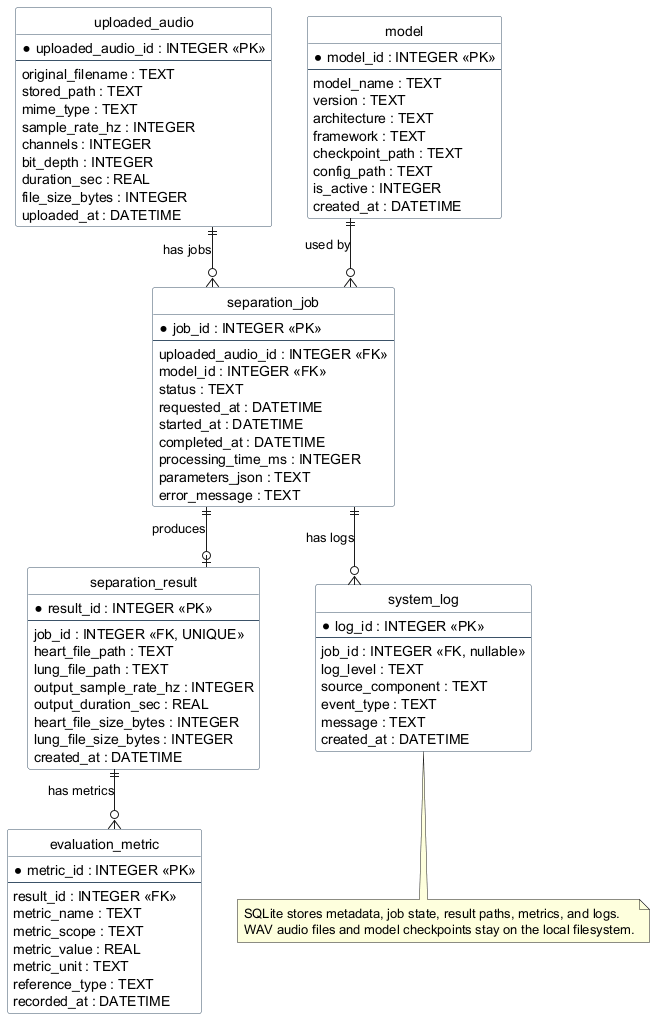
\includegraphics[width=0.82\textwidth]{erd.png}
  \caption{Entity Relationship Diagram}
  \label{fig:erd}
\end{figure}

Figure~\ref{fig:erd} shows the SQLite database structure used to store structured project data. The \texttt{uploaded\_audio} table records each uploaded WAV file, the \texttt{model} table records available model information, and the \texttt{separation\_job} table connects an uploaded file with the model used for processing. The \texttt{separation\_result} table stores the paths and metadata for generated heart and lung outputs.

The design intentionally stores file paths and metadata in SQLite rather than storing large WAV audio blobs in the database. This supports a practical student project architecture: local storage keeps uploaded and generated audio files, while SQLite supports history, result lookup, job status, metrics, and logs. As a result, the browser can display previous jobs and download links without scanning folders manually.

\section{Object Diagram}

\begin{figure}[H]
  \centering
  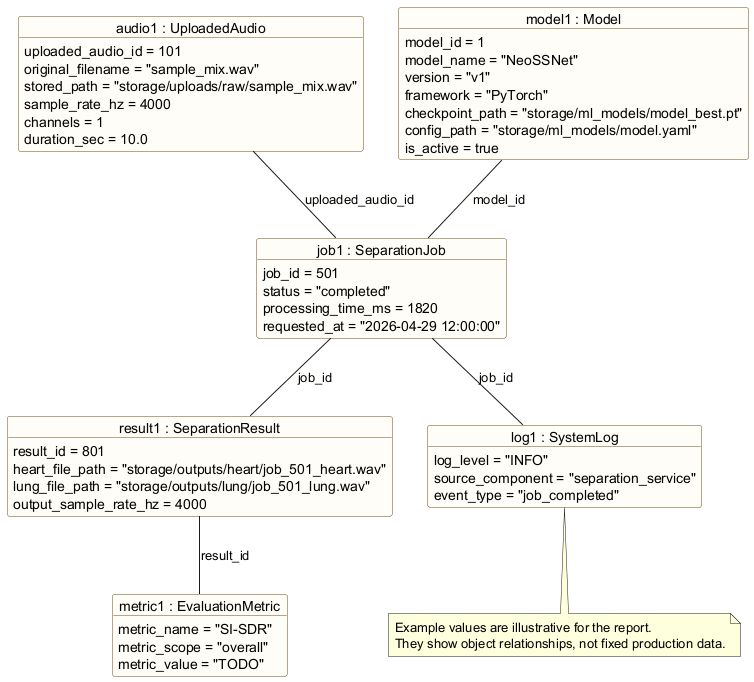
\includegraphics[width=0.88\textwidth]{object_diagram.png}
  \caption{Object Diagram for a Completed Separation Job}
  \label{fig:object-diagram}
\end{figure}

Figure~\ref{fig:object-diagram} gives a concrete example of how the system data may look after one successful separation. One \texttt{UploadedAudio} object is linked to one \texttt{SeparationJob}, the job uses an active \texttt{Model}, and the completed job produces a \texttt{SeparationResult} containing heart and lung output file paths.

The object diagram helps explain how upload, separation, storage, result viewing, and history are connected at runtime. When a user views history, the system can retrieve the job, original upload metadata, model information, output paths, optional metrics, and log record as related objects. This gives the project a traceable flow from the original mixed input to the separated outputs.

\chapter{Requirements}

This chapter defines the main functional requirements, non-functional requirements, software design concepts, and design principles for the cardiopulmonary sound separation system. The system is treated as a prototype and proof of concept for a software design assignment and Final Year Project context. It is designed to demonstrate a realistic local web application that can upload mixed cardiopulmonary audio, run NeoSSNet-based separation, store metadata, and present results clearly to students, lecturers, researchers, or demonstration users. The requirements do not claim clinical validation; they focus on software behaviour, maintainability, and demonstration readiness.

\section{Functional Requirements}

Functional requirements describe the main behaviours that the system must provide to the user and to the backend workflow.

\begin{table}[H]
  \centering
  \small
  \caption{Functional Requirements}
  \label{tab:functional-requirements}
  \begin{tabularx}{\textwidth}{p{0.12\textwidth} p{0.25\textwidth} Y}
    \toprule
    \textbf{ID} & \textbf{Requirement} & \textbf{Description} \\
    \midrule
    FR-01 & Upload mixed WAV audio & The user shall be able to select and upload a mixed cardiopulmonary WAV file through the web interface. \\
    FR-02 & Validate audio file & The backend shall check that the uploaded file is a valid supported audio file before saving it for processing. \\
    FR-03 & Run cardiopulmonary sound separation & The backend shall run the separation workflow using NeoSSNet to separate the mixed input into heart and lung sound outputs. \\
    FR-04 & Generate heart and lung output files & The system shall save separated heart and lung audio files in the configured output folders. \\
    FR-05 & Preview separated audio & The web interface shall allow the user to preview the original audio and the separated heart and lung outputs where browser playback is supported. \\
    FR-06 & Download separated audio & The user shall be able to download the generated heart and lung output files for later review or demonstration. \\
    FR-07 & View processing history & The system shall show previous uploads, jobs, statuses, and result links so that users can review earlier processing activity. \\
    FR-08 & Store logs and metadata & The system shall store upload metadata, job records, result paths, metrics where available, and important processing logs in SQLite. \\
    \bottomrule
  \end{tabularx}
\end{table}

These functional requirements support the main demonstration flow of the project. A user uploads a mixed sound, the backend validates and processes it, the system stores the generated files, and the browser presents previews, downloads, and history. This keeps the project focused on a working end-to-end software system rather than only a standalone machine learning script.

\section{Non-Functional Requirements}

Non-functional requirements describe the quality attributes expected from the prototype. These qualities are important because the system should be understandable, maintainable, and reliable enough for local testing and presentation.

\begin{table}[H]
  \centering
  \small
  \caption{Non-Functional Requirements}
  \label{tab:non-functional-requirements}
  \begin{tabularx}{\textwidth}{p{0.24\textwidth} Y}
    \toprule
    \textbf{Quality Attribute} & \textbf{Requirement} \\
    \midrule
    Usability & The interface should make the upload, separation, preview, download, and history flow clear for a student or examiner during a demonstration. \\
    Maintainability & The code should be organised into clear frontend, router, service, machine learning, database, and storage responsibilities so that future changes are easier to make. \\
    Reliability & The backend should handle invalid files, failed separation jobs, missing outputs, and database errors with clear status messages and logs. \\
    Modularity & Each major part of the system should be replaceable or testable with minimal impact on unrelated components. \\
    Performance & The system should process short demonstration WAV files within a reasonable time on a local machine, while avoiding unnecessary database storage of large audio blobs. \\
    Data integrity & SQLite records should consistently link uploaded audio, model records, separation jobs, results, metrics, and logs. Failed jobs should keep useful error information. \\
    Portability and local execution & The system should run locally using Python, FastAPI, SQLite, PyTorch, and local folders without requiring cloud services or complex deployment infrastructure. \\
    \bottomrule
  \end{tabularx}
\end{table}

The non-functional requirements guide implementation decisions. For example, local execution supports a practical student project setup, while data integrity and logging support traceability when explaining how a mixed input becomes separated heart and lung outputs.

\section{Software Design Concepts}

\subsection{Abstraction}

Abstraction is used to hide detailed processing steps behind simpler operations. In this project, the separation route does not need to know how model records are selected, how NeoSSNet is called, or how heart and lung output paths are written. It can call a service-level operation such as \texttt{separate\_uploaded\_audio} and treat the workflow as one meaningful software action.

The machine learning boundary also uses abstraction. \texttt{SeparationAlgorithm} represents the expected behaviour of a separation model, while \texttt{NeoSSNetStrategy} provides the current real implementation. This allows the service layer to express the workflow in terms of cardiopulmonary sound separation rather than in terms of one concrete model class.

\subsection{Modularity}

Modularity divides the system into smaller parts with clear responsibilities. The frontend handles upload controls, audio preview, download links, and history display. FastAPI routers handle HTTP requests. Services coordinate workflows. The ML layer performs real separation. SQLite models store structured records, and local folders store uploaded and generated WAV files.

This modular structure is useful for the prototype because a change in one area does not require rewriting the entire system. For example, improving the frontend model dropdown should not require changing NeoSSNet inference, and changing output folder naming should not require changing the database schema.

\subsection{Separation of Concerns}

Separation of concerns prevents unrelated responsibilities from being mixed together. The upload route receives files, the storage service manages local file placement, the model service reads available model records, the separation service coordinates processing, and the ML strategy runs inference. This keeps web request handling, file management, model selection, and audio separation as separate concerns.

The same idea applies to data storage. Runtime upload folders, generated output folders, model checkpoints, dataset folders, and SQLite metadata serve different purposes and remain separate. This design avoids training from runtime upload folders and avoids storing large WAV content directly in SQLite.

\subsection{Information Hiding}

Information hiding means that internal implementation details are kept inside the module or class responsible for them. File validation and path rules should stay inside upload or storage-related code. Model selection rules should stay inside \texttt{ModelService}. Algorithm construction should stay inside \texttt{SeparationAlgorithmFactory}. NeoSSNet inference details should stay inside the ML strategy and inference function.

This protects the rest of the system from unnecessary implementation knowledge. For example, the route does not need to know where the checkpoint file is stored or how the strategy calls the underlying inference function; it only needs the job result returned by the service.

\subsection{Low Coupling and High Cohesion}

Low coupling means that components should depend on each other only where necessary. In this project, \texttt{SeparationService} depends on the \texttt{SeparationAlgorithm} abstraction rather than depending directly on NeoSSNet-specific workflow logic. This reduces the impact of future model changes because the upload, result, history, and download routes can remain stable.

High cohesion means that each component should focus on related tasks. \texttt{StorageService} is cohesive when it handles file storage concerns, \texttt{ModelService} is cohesive when it handles model lookup, and \texttt{NeoSSNetStrategy} is cohesive when it only adapts NeoSSNet inference to the shared algorithm interface. Cohesion helps the system remain easy to explain and test.

\section{Design Principles}

\subsection{Single Responsibility Principle}

The Single Responsibility Principle supports the assignment of one main reason for change to each component. For example, \texttt{StorageService} should change when file storage rules change, not when separation model logic changes. This keeps file handling separate from ML inference and database workflow decisions.

\begin{lstlisting}[caption={Single Responsibility Principle Example}]
# Single Responsibility Principle:
# StorageService handles storage concerns only.
class StorageService:
    def save_uploaded_wav(self, upload_file) -> str:
        stored_path = build_upload_path(upload_file.filename)
        write_file(upload_file, stored_path)
        return stored_path


# Request handling remains outside StorageService.
def upload_audio_route(file, db):
    stored_path = StorageService().save_uploaded_wav(file)
    return create_uploaded_audio_record(db, file.filename, stored_path)
\end{lstlisting}

In this example, the storage class does not create separation jobs and does not run NeoSSNet. Its responsibility is limited to saving files and returning a path that other components can use.

\subsection{Open/Closed Principle}

The Open/Closed Principle suggests that the system should be open for extension but closed for unnecessary modification. The separation workflow should be able to support a new implemented algorithm by adding a strategy class and registering it in the factory, without rewriting upload, result, history, or download routes.

\begin{lstlisting}[caption={Open/Closed Principle Example}]
# Open for extension:
# add a new implemented strategy and register it in the factory.
class NeoSSNetStrategy:
    def separate(self, input_wav_path, model_path, config_path,
                 heart_output_path, lung_output_path):
        return run_neossnet_inference(...)


class SeparationAlgorithmFactory:
    _registry = {
        "neossnet": NeoSSNetStrategy,
    }

    @classmethod
    def create(cls, model):
        strategy_class = cls._registry[model.architecture.lower()]
        return strategy_class()
\end{lstlisting}

The workflow is closed to unnecessary modification because \texttt{SeparationService} can keep the same high-level steps. A future algorithm should mainly require a new concrete strategy and a factory registration.

\subsection{Dependency Inversion Principle}

Dependency Inversion is relevant because high-level workflow classes should not be tightly bound to one concrete model implementation. \texttt{SeparationService} should depend on the \texttt{SeparationAlgorithm} abstraction, while \texttt{NeoSSNetStrategy} provides the current concrete implementation.

\begin{lstlisting}[caption={Dependency Inversion Principle Example}]
# Dependency Inversion Principle:
# high-level workflow depends on the abstraction.
class SeparationService:
    def run_algorithm(self, algorithm: SeparationAlgorithm, paths):
        return algorithm.separate(
            input_wav_path=paths.input_wav,
            model_path=paths.model_checkpoint,
            model_config_path=paths.model_config,
            heart_output_path=paths.heart_output,
            lung_output_path=paths.lung_output,
        )
\end{lstlisting}

The service does not need to instantiate or know the internal details of \texttt{NeoSSNetStrategy}. The factory supplies an object that satisfies the \texttt{SeparationAlgorithm} interface, and the service runs the workflow through that abstraction.

\subsection{Interface-Based Design for Algorithm Replacement}

Interface-based design supports future algorithm replacement by defining the expected input and output of a separation algorithm. The current algorithm should produce separated heart and lung audio outputs, but the service layer should not need to know whether the implementation uses NeoSSNet, an ONNX-exported model, or a future baseline method. For the current project, NeoSSNet remains the required real separation model.

\subsection{Persistence Separation Between SQLite and Filesystem}

The design separates structured metadata from large binary audio files. SQLite stores records such as filenames, file paths, upload timestamps, job status, model information, output paths, metrics, and logs. The filesystem stores uploaded WAV files, generated heart and lung outputs, model checkpoints, and dataset files. This approach is simpler to run locally and avoids making the database unnecessarily large.

\section{Software Design Plan}

The proposed software design is organised into layers. This layered plan supports a clear implementation path and makes the system easier to explain in the report and viva presentation.

\begin{table}[H]
  \centering
  \small
  \caption{Software Design Plan by Layer}
  \label{tab:software-design-plan}
  \begin{tabularx}{\textwidth}{p{0.24\textwidth} p{0.30\textwidth} Y}
    \toprule
    \textbf{Layer} & \textbf{Main Responsibility} & \textbf{Project Role} \\
    \midrule
    Frontend layer & HTML, CSS, JavaScript, templates, and browser audio controls & Provides upload form, status messages, original and separated audio playback, download links, and history display. \\
    Backend API layer & FastAPI application and routers & Receives upload, separation, result, download, history, log, and health requests. \\
    Service layer & Workflow coordination and business logic & Connects validation, database updates, NeoSSNet inference, output storage, logging, and result retrieval. \\
    ML inference layer & Audio preprocessing and model inference & Loads or prepares audio, applies the NeoSSNet model, and returns separated heart and lung waveforms. \\
    Database layer & SQLite schema and repository-style access & Stores uploaded audio metadata, model records, job states, result paths, metrics, and system logs. \\
    Storage layer & Local filesystem folders & Stores uploaded mixed WAV files, temporary files, separated heart and lung outputs, logs where needed, and ML model weights. \\
    \bottomrule
  \end{tabularx}
\end{table}

The design plan follows the project priority of real functionality first, then simplicity and local execution. It avoids unnecessary cloud, microservice, or authentication complexity unless those features are explicitly added later.

\chapter{Proposed Design Patterns}
\sloppy

This chapter proposes three design patterns for the cardiopulmonary sound separation system. The patterns are presented as practical backend design structures for the FastAPI, SQLite, local storage, and NeoSSNet pipeline. Each pattern is linked to a specific project problem so that the design remains useful for implementation and explanation during the final presentation.

The class and method names used in this chapter represent the proposed backend design. During implementation, they should be kept aligned with the final source code while preserving the same responsibilities and pattern roles.

\section{Facade Pattern}

The Facade Pattern is proposed to provide a simple interface over the separation workflow, which contains several lower-level operations such as audio preprocessing, model inference, file storage, database updates, and logging \parencite{gamma1994designpatterns}.

\subsection{Pattern Type}

The Facade Pattern is a structural design pattern. It focuses on arranging classes so that a client can access a complex subsystem through a simpler and more stable interface.

\subsection{Problem}

The separation endpoint should not directly coordinate every step of the backend workflow. If the FastAPI router directly calls the audio preprocessor, NeoSSNet inference class, storage utilities, database session, and logging logic, the route becomes difficult to read, test, and modify. This would also make the design harder to explain because web routing logic and machine learning workflow logic would be mixed in one place.

\subsection{Solution}

The proposed solution is to introduce \texttt{SeparationService} as the facade. The router calls one high-level method, such as \texttt{run\_separation(audio\_id)}, while the service coordinates the subsystem classes internally. This keeps the router focused on request handling and keeps the separation workflow inside a dedicated service layer.

\subsection{Structure}

The template structure below shows how a facade sits between a client and a group of subsystem classes. The client depends on the facade instead of depending on each subsystem class directly.

\begin{figure}[H]
  \centering
  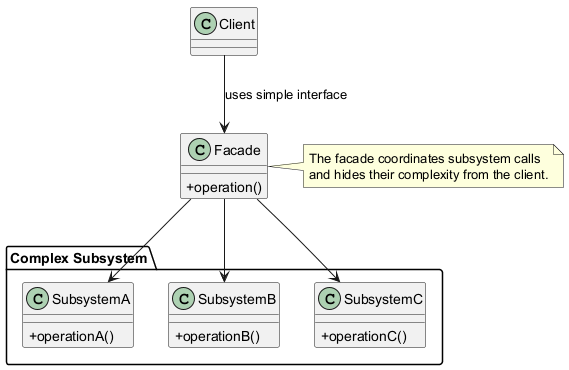
\includegraphics[width=0.82\textwidth]{facade_template.png}
  \caption{Facade Pattern Template Structure}
  \label{fig:facade-template}
\end{figure}

\begin{enumerate}
  \item \textbf{Client:} The external caller that needs to use the subsystem. In this project, the client is mainly the FastAPI router that receives a separation request.
  \item \textbf{Facade:} The simplified interface used by the client. In this project, \texttt{SeparationService} hides the detailed separation steps behind one service method.
  \item \textbf{Additional Facade:} An optional second facade can be used when the subsystem grows. For example, a future \texttt{ModelManagementService} could hide model loading and model version selection if that logic becomes large.
  \item \textbf{Complex Subsystem:} The lower-level classes that perform the actual work. In this project, these include audio preprocessing, NeoSSNet inference, storage handling, database updates, and system logging.
\end{enumerate}

\subsection{Project Application}

\subsubsection{i. Function or Software Component Affected}

The affected component is the backend separation workflow, especially the service layer that connects the FastAPI separation route to the audio and machine learning components. The proposed main class is \texttt{SeparationService}. The route module may be named \texttt{separation.py} or another consistent router name in the final implementation.

\subsubsection{ii. Description of Workflow or Data Flow}

The router receives a request to separate an uploaded WAV file. It passes the uploaded audio identifier to \texttt{SeparationService}. The service loads the upload metadata from SQLite, reads the audio file from local storage, preprocesses it into the expected model input format, runs NeoSSNet inference, saves the separated heart and lung audio files, updates the separation result in SQLite, and writes important processing events to the log.

\subsubsection{iii. Sample Class Diagram}

\begin{figure}[H]
  \centering
  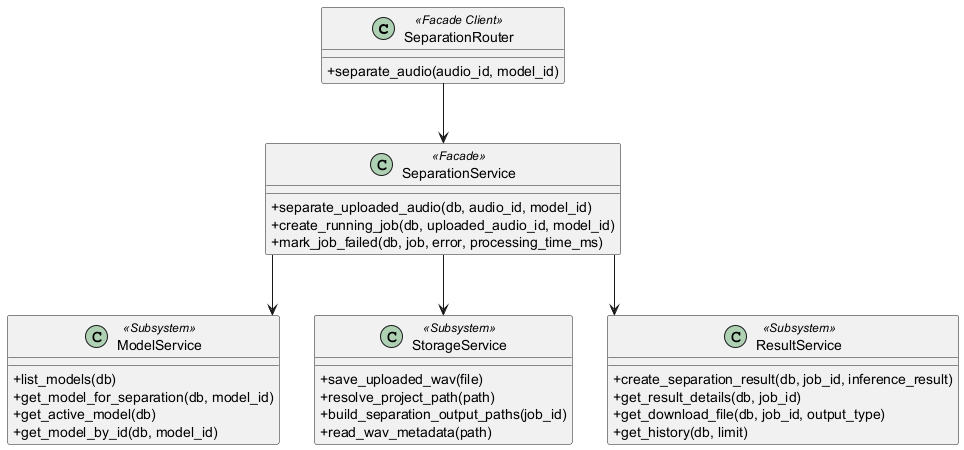
\includegraphics[width=\textwidth]{facade_project.png}
  \caption{Facade Pattern Project Class Diagram}
  \label{fig:facade-project}
\end{figure}

\subsubsection{iv. Sample Other UML Notation}

\begin{figure}[H]
  \centering
  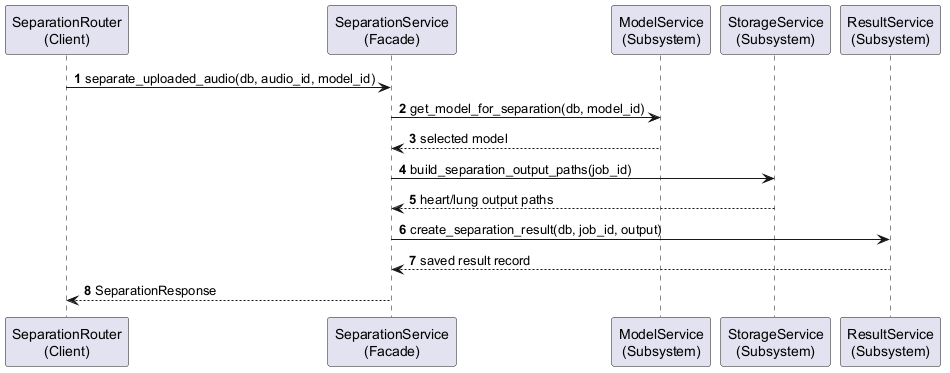
\includegraphics[width=\textwidth]{facade_sequence.png}
  \caption{Facade Pattern Sequence Diagram}
  \label{fig:facade-sequence}
\end{figure}

\subsubsection{v. Sample Potential Code}

\begin{verbatim}
class SeparationService:
    def __init__(
        self,
        preprocessor,
        inference,
        storage,
        repository,
        logger,
    ):
        self.preprocessor = preprocessor
        self.inference = inference
        self.storage = storage
        self.repository = repository
        self.logger = logger

    def run_separation(self, audio_id: int) -> int:
        upload = self.repository.get_uploaded_audio(audio_id)
        waveform = self.preprocessor.load_and_prepare(upload.file_path)
        heart, lung = self.inference.separate(waveform)
        output_paths = self.storage.save_outputs(audio_id, heart, lung)
        job_id = self.repository.save_result(audio_id, output_paths)
        self.logger.info(job_id, "Separation completed")
        return job_id
\end{verbatim}

The code sample is illustrative and should be aligned with the final backend method names during implementation.

\subsubsection{vi. Benefits}

The facade makes the route simpler, improves separation of concerns, and makes the workflow easier to test as one service operation. It also improves presentation clarity because the main separation process can be explained as a single service call that coordinates several internal components.

\subsubsection{vii. Limitations}

The main limitation is that the facade can become too large if every processing rule is placed inside \texttt{SeparationService}. The implementation should keep detailed work inside subsystem classes and use the facade mainly for orchestration.

\section{Strategy Pattern}

The Strategy Pattern is proposed to keep the separation algorithm interchangeable behind a common interface. This is useful because the project currently focuses on NeoSSNet, but future versions may compare another PyTorch model, an ONNX-exported model, or a simple baseline method \parencite{gamma1994designpatterns}.

\subsection{Pattern Type}

The Strategy Pattern is a behavioral design pattern. It focuses on defining a family of algorithms and allowing the context object to use them through a shared interface.

\subsection{Problem}

The system should not hardcode NeoSSNet-specific logic throughout the service layer. If model-specific preprocessing, inference, and output handling are tightly coupled to the route or service, future experiments become harder. Even for a student project, keeping the algorithm boundary clear makes the design easier to test and explain.

\subsection{Solution}

The proposed solution is to define a \texttt{SeparationAlgorithm} interface with a method such as \texttt{separate(waveform)}. \texttt{NeoSSNetStrategy} becomes the current concrete strategy. \texttt{SeparationService} acts as the context and calls the selected strategy through the shared interface.

\subsection{Structure}

The template structure below shows a context object that delegates algorithm-specific work to a strategy object. The client uses the context without needing to know which concrete strategy performs the work.

\begin{figure}[H]
  \centering
  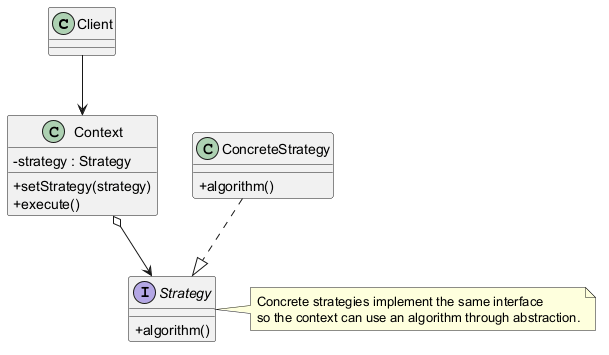
\includegraphics[width=0.82\textwidth]{strategy_template.png}
  \caption{Strategy Pattern Template Structure}
  \label{fig:strategy-template}
\end{figure}

\begin{enumerate}
  \item \textbf{Context:} The object that uses a strategy to complete part of its work. In this project, \texttt{SeparationService} is the context because it delegates model-specific separation to an algorithm object.
  \item \textbf{Strategy Interface:} The common contract for all algorithms. In this project, \texttt{SeparationAlgorithm} defines the expected separation method and output format.
  \item \textbf{Concrete Strategies:} The actual algorithm implementations. \texttt{NeoSSNetStrategy} is the main strategy, while \texttt{ONNXNeoSSNetStrategy} or \texttt{BaselineSeparationStrategy} can be considered future options.
  \item \textbf{Client:} The caller that starts the workflow. In this project, the FastAPI router starts the separation request, while the service uses the configured strategy internally.
\end{enumerate}

\subsection{Project Application}

\subsubsection{i. Function or Software Component Affected}

The affected component is the machine learning inference boundary. The main classes are \texttt{SeparationAlgorithm}, \texttt{NeoSSNetStrategy}, and \texttt{SeparationService}. Alternative strategies are treated as future extensions unless they are implemented in the final backend.

\subsubsection{ii. Description of Workflow or Data Flow}

The service receives a prepared waveform from the preprocessing step. Instead of calling a NeoSSNet class directly throughout the workflow, it calls the selected \texttt{SeparationAlgorithm}. The current concrete strategy runs NeoSSNet and returns two outputs: the separated heart sound and the separated lung sound. The rest of the workflow can then save and record the outputs without depending on the internal details of the selected algorithm.

\subsubsection{iii. Sample Class Diagram}

\begin{figure}[H]
  \centering
  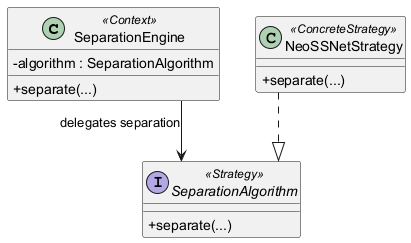
\includegraphics[width=\textwidth]{strategy_project.png}
  \caption{Strategy Pattern Project Class Diagram}
  \label{fig:strategy-project}
\end{figure}

\subsubsection{iv. Sample Other UML Notation}

\begin{figure}[H]
  \centering
  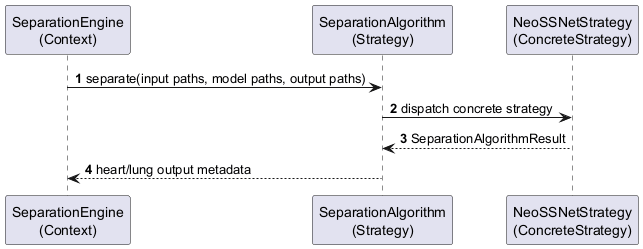
\includegraphics[width=\textwidth]{strategy_sequence.png}
  \caption{Strategy Pattern Sequence Diagram}
  \label{fig:strategy-sequence}
\end{figure}

\subsubsection{v. Sample Potential Code}

\begin{verbatim}
from abc import ABC, abstractmethod


class SeparationAlgorithm(ABC):
    @abstractmethod
    def separate(self, waveform):
        raise NotImplementedError


class NeoSSNetStrategy(SeparationAlgorithm):
    def __init__(self, model):
        self.model = model

    def separate(self, waveform):
        heart, lung = self.model.predict(waveform)
        return heart, lung


class SeparationService:
    def __init__(self, algorithm: SeparationAlgorithm):
        self.algorithm = algorithm

    def separate_waveform(self, waveform):
        return self.algorithm.separate(waveform)
\end{verbatim}

The \texttt{model.predict} call is a simplified placeholder for the final PyTorch inference method used by NeoSSNet.

\subsubsection{vi. Benefits}

The strategy design makes the algorithm boundary clear, improves testability, and supports future comparison with alternative separation methods. It also helps keep NeoSSNet-specific code inside a dedicated class rather than spreading it across the router and service layer.

\subsubsection{vii. Limitations}

The limitation is that the project may only use NeoSSNet during the final submission. If no alternative algorithm is implemented, the extra interface should remain small so it does not make the student project unnecessarily complicated.

\section{Factory Method Pattern}

The Factory Method Pattern is proposed to centralise the creation of separation algorithm objects. This avoids scattering model creation, checkpoint loading, and strategy selection logic throughout the backend \parencite{gamma1994designpatterns}.

\subsection{Pattern Type}

The Factory Method Pattern is a creational design pattern. It focuses on creating objects through a dedicated creator method instead of directly constructing concrete classes in client code.

\subsection{Problem}

The system stores model-related information such as model name, version, checkpoint path, and active status in SQLite or local configuration. If each service directly constructs \texttt{NeoSSNetStrategy} and loads checkpoint paths manually, model creation becomes duplicated and harder to change. This is especially risky if the project later supports more than one model format.

\subsection{Solution}

The proposed solution is to use \texttt{SeparationAlgorithmFactory} as the creator. The factory reads the active model configuration or receives it from the service, then returns a \texttt{SeparationAlgorithm} object. At the current stage, the main concrete product is \texttt{NeoSSNetStrategy}.

\subsection{Structure}

The template structure below shows a creator that returns a product interface while hiding the exact concrete product class from the client.

\begin{figure}[H]
  \centering
  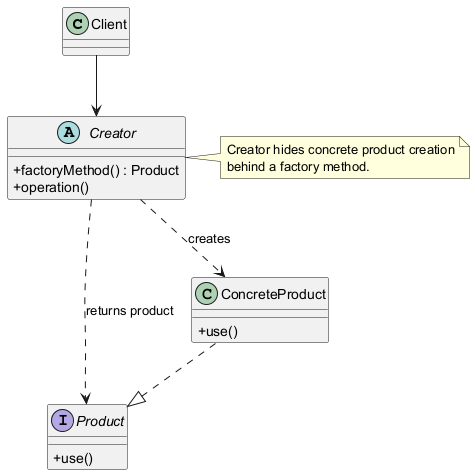
\includegraphics[width=0.82\textwidth]{factory_method_template.png}
  \caption{Factory Method Pattern Template Structure}
  \label{fig:factory-method-template}
\end{figure}

\begin{enumerate}
  \item \textbf{Creator:} The class or method responsible for creating product objects. In this project, \texttt{SeparationAlgorithmFactory} is the proposed creator.
  \item \textbf{Concrete Creator:} The specific creation logic that knows which concrete product to instantiate. In this project, the factory method can create a NeoSSNet-based strategy from the active model configuration.
  \item \textbf{Product:} The shared interface returned to the client. In this project, \texttt{SeparationAlgorithm} is the product interface.
  \item \textbf{Concrete Product:} The actual object created by the factory. In this project, \texttt{NeoSSNetStrategy} is the main concrete product.
  \item \textbf{Client:} The class that requests a product from the factory. In this project, \texttt{SeparationService} uses the factory so that it does not need to hardcode model construction details.
\end{enumerate}

\subsection{Project Application}

\subsubsection{i. Function or Software Component Affected}

The affected component is model and algorithm construction. The main proposed class is \texttt{SeparationAlgorithmFactory}, used by \texttt{SeparationService}. A shorter name such as \texttt{ModelFactory} can be used in implementation if the responsibility remains clear.

\subsubsection{ii. Description of Workflow or Data Flow}

The service requests the active separation algorithm from the factory. The factory checks the model configuration, such as model type and checkpoint path, and creates the matching algorithm object. The created object is returned through the \texttt{SeparationAlgorithm} interface. The service then calls the algorithm without knowing the exact construction steps.

\subsubsection{iii. Sample Class Diagram}

\begin{figure}[H]
  \centering
  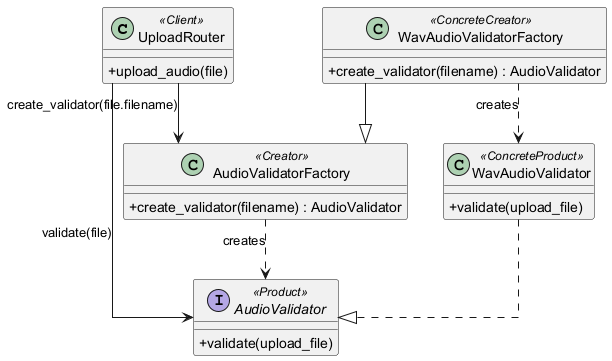
\includegraphics[width=\textwidth]{factory_method_project.png}
  \caption{Factory Method Pattern Project Class Diagram}
  \label{fig:factory-method-project}
\end{figure}

\subsubsection{iv. Sample Other UML Notation}

\begin{figure}[H]
  \centering
  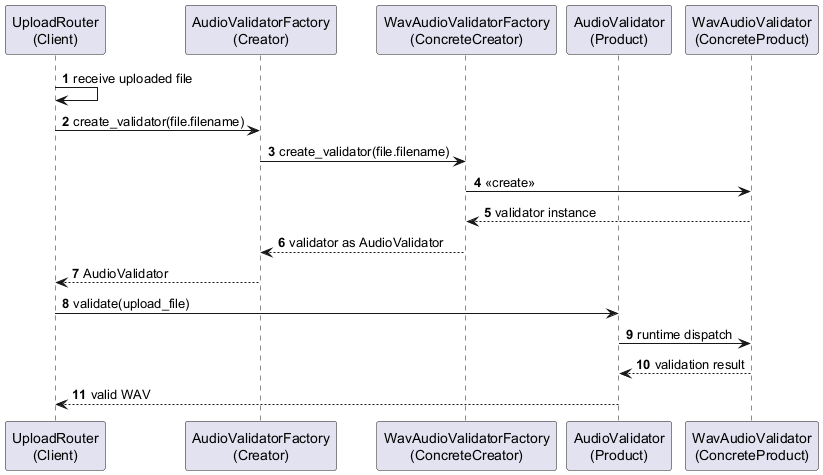
\includegraphics[width=\textwidth]{factory_method_sequence.png}
  \caption{Factory Method Pattern Sequence Diagram}
  \label{fig:factory-method-sequence}
\end{figure}

\subsubsection{v. Sample Potential Code}

\begin{verbatim}
class SeparationAlgorithmFactory:
    def create(self, model_config) -> SeparationAlgorithm:
        if model_config.model_type == "neossnet":
            checkpoint = model_config.checkpoint_path
            model = load_neossnet_checkpoint(checkpoint)
            return NeoSSNetStrategy(model)

        message = f"Unsupported model type: {model_config.model_type}"
        raise ValueError(message)


class SeparationService:
    def __init__(
        self,
        factory: SeparationAlgorithmFactory,
        model_repository,
    ):
        self.factory = factory
        self.model_repository = model_repository

    def get_algorithm(self):
        active_model = self.model_repository.get_active_model()
        return self.factory.create(active_model)
\end{verbatim}

The \texttt{load\_neossnet\_checkpoint} call represents the final model loading function used by the project.

\subsubsection{vi. Benefits}

The factory method reduces hardcoded model creation, keeps checkpoint loading in one place, and makes it easier to add a future model type without changing every service that needs an algorithm. It also supports cleaner testing because a test can provide a simple model configuration and check which strategy is created.

\subsubsection{vii. Limitations}

The limitation is that a factory may be unnecessary if the system permanently supports only one model. For this project, the factory should stay small and practical, mainly to keep model construction clear and centralised.
\fussy

\chapter{Conclusion and Suggestions}

\section{Conclusion}

This report proposed the design of a HealthTech cardiopulmonary sound separation system as a prototype and proof of concept. The system is intended to accept mixed WAV audio, run cardiopulmonary sound separation, and produce separate heart sound and lung sound output files. It supports the main user workflow of upload, validation, separation, preview, download, and processing history while keeping the implementation practical for a student software design project.

The proposed architecture is important because the machine learning model is only one part of the complete system. FastAPI provides the backend API layer for handling upload, separation, result, download, and history requests. NeoSSNet provides the core separation model for generating heart and lung audio outputs. SQLite stores structured metadata such as uploaded audio records, model details, separation jobs, result paths, evaluation metrics, and logs. Local storage keeps the actual uploaded WAV files, separated output files, and model weights, which avoids storing large audio content directly inside the database.

The selected design patterns strengthen the proposed design. The Facade Pattern simplifies the separation workflow by allowing the separation router to call a high-level service instead of directly managing model lookup, storage paths, result records, and database updates. The Strategy Pattern keeps algorithm execution inside \texttt{SeparationEngine}, which depends on the \texttt{SeparationAlgorithm} abstraction while \texttt{NeoSSNetStrategy} wraps the real NeoSSNet inference path. The Factory Method Pattern is used in model-selection support, where \texttt{SeparationAlgorithmFactory} creates the correct \texttt{SeparationAlgorithm} strategy from the selected SQLite \texttt{Model} record before the engine runs separation.

Overall, the proposed design demonstrates how machine learning, database persistence, local file storage, and web interaction can be organised into a reusable software system. The report does not claim clinical validation or real hospital deployment. Instead, it presents a clear and maintainable software design suitable for assignment submission, demonstration, and future implementation improvement.

\section{Suggestions / Future Work}

Several improvements can be considered after the core prototype is working:

\begin{enumerate}
  \item \textbf{Improve frontend usability:} The user interface can be refined with clearer progress indicators, better error messages, improved history filtering, and more polished audio playback controls.
  \item \textbf{Add more datasets and noise conditions:} Future testing can include broader cardiopulmonary recordings, different noise levels, and additional real-world recording conditions to better understand model behaviour.
  \item \textbf{Add asynchronous or background processing:} Longer audio files or slower inference tasks can be handled using background jobs so that the web request does not need to wait synchronously for the full separation process.
  \item \textbf{Add authentication if needed:} If the system is extended beyond a local demonstration, user login and role-based access can be added to protect uploaded files and processing history.
  \item \textbf{Add algorithms through Strategy:} Alternative approaches, baseline methods, or future ONNX-based versions can be added as new strategies without changing the main router workflow.
  \item \textbf{Improve evaluation metrics and reporting:} The system can provide clearer metric reports such as SNR, SDR, SI-SDR, MSE, or MAE where suitable reference data is available.
  \item \textbf{Validate on broader real-world recordings:} Further validation should be performed on more varied recordings before making any claim about robustness or clinical usefulness.
\end{enumerate}

In conclusion, the project provides a strong foundation for a practical software design around cardiopulmonary sound separation. Its main value is not only the use of NeoSSNet, but also the structured design that makes upload handling, inference, storage, logging, result viewing, and future extension easier to understand and maintain.


\begingroup
\sloppy
\printbibliography[heading=bibintoc,title={Bibliography / References}]
\endgroup

\end{document}
